% =====================================================================
%  Divergence of EF21-SignMuon (Theorem th:ef_div).
%  Drop-in appendix subsection for v2_SignMuon_AAAI.tex (double-column).
%  Structure: Theorem -> Proof idea (narrative) -> Proof in three labelled
%  parts (rescaling; the limit cycle; the realization).  Exact rational
%  arithmetic; the construction and its all-method comparison are implemented
%  in code/counterexamples/problems.py (figure via run_counterexamples.py).
% =====================================================================
\providecommand{\smat}[4]{\bigl(\begin{smallmatrix}#1&#2\\#3&#4\end{smallmatrix}\bigr)}

\subsection{Proof of Theorem~\ref{th:ef_div} (Divergence of EF21-SignMuon)}\label{app:proof_th4}

% The statement is repeated here for the reader. The counter is set by hand so
% that the restatement carries the main text's number 4 and does not consume a
% new one; ef21_musign_reduction.tex sets it again for Theorem 5. No \label is
% attached: th:ef_div stays the main-text statement.
\setcounter{theorem}{3}
\begin{theorem}[Divergence of EF21-SignMuon]
For every $L>0$, step size $\eta>0$, momentum coefficient $\mu\in[0,1)$, and
either momentum variant, there is an $L$-smooth (Assumption~\ref{as:2}),
bounded-below (Assumption~\ref{as:1}) function
$f:\mathbb{R}^{2\times2}\!\to\mathbb{R}$ on which EF21-SignMuon started at
$\mathbf{X}_0=\mathbf{0}$ diverges: for an explicit constant $c=c(f)>0$,
\begin{equation}\label{eq:exact_rate_app}
f(\mathbf{X}_{t+2})-f(\mathbf{X}_t)=c\,L\eta^2>0\qquad(t\ge3),
\end{equation}
so $f(\mathbf{X}_t)\to+\infty$. In particular, no step-size rule
$\eta=\eta(L,\mu)$ using only the smoothness and momentum constants can make
the method convergent.
\end{theorem}

Recall from the main text that EF21-SignMuon (Algorithm~\ref{ef21_signmuon})
does not descend along the LMO output
$\mathbf D_t=\operatorname{polar}(\tilde{\mathbf M}_t)$ itself, but along the
error-feedback estimate $\mathbf d_t^{\mathrm{est}}$ of \eqref{eq:efsm_est},
followed by $\mathbf X_t=\mathbf X_{t-1}-\eta\,\mathbf d_t^{\mathrm{est}}$. A
\emph{single} magnitude $\alpha_t$ rescales the signs of \emph{all} entries at
once, and it is this coupling that the counterexample exploits. We now prove
Theorem~\ref{th:ef_div}.

\subsubsection*{Proof idea}

\emph{The mechanism.} The error-feedback update \eqref{eq:efsm_est} moves
\emph{every} entry of $\mathbf d_t^{\mathrm{est}}$ by the same magnitude
$\alpha_t$; only the signs are individual. Suppose then that one entry must
track a target alternating
between $+1$ and $-1$ while another must track a small constant
$-\varepsilon$. The alternating entry keeps its residual, and with it
$\alpha_t$, at $\Theta(1)$; the constant entry is therefore displaced by
$\pm\Theta(1)$ at every step and can only oscillate about its target, never
settle on it. Which side of the target the oscillation favours is decided by
its \emph{phase}, and a one-bit sign carries no information by which a phase
could be corrected. In the unfavourable phase the estimate of the constant
entry has a time average of the sign \emph{opposite} to $-\varepsilon$, and
the iterate driven by that estimate moves the wrong way forever.

\emph{From the sketch to an instance.} The sketch is not yet a counterexample:
in EF21-SignMuon the quantity tracked is the LMO output
$\mathbf D_t=\operatorname{polar}(\tilde{\mathbf M}_t)$, a polar factor of
unit spectral norm, and the gradients behind it must all come from one smooth
function. Both constraints are met at size $2\times2$ by the reflections
$\bar{\mathbf D}^{\pm}=\smat{a}{\pm b}{\pm b}{-a}$ with $a^2+b^2=1$: one
matrix the oracle can emit carries both roles of the sketch at once, the
large alternating entries on the off-diagonal ($b=\tfrac{24}{25}$) and the
small constant ones on the diagonal ($a=\tfrac7{25}$), coupled by the shared
$\alpha_t$. On these targets the estimate enters a period-two cycle in which
the time average of the $(2,2)$-entry is positive although every target value
is $-\tfrac7{25}$, so $(\mathbf X_t)_{22}$ travels to $-\infty$, the direction
in which the objective increases (Figure~\ref{fig:divergence_plot}, right). Nor does the mechanism rest on
degeneracy: the momentum matrices of the divergent tail have condition number
$\tfrac{16}{9}$ throughout.

\emph{The role of the preamble.} The unfavourable phase must be arranged.
From $\mathbf d_0^{\mathrm{est}}=\mathbf 0$, the alternating targets alone
lock the estimate into a period-two cycle whose diagonal average has the
\emph{correct} sign. The recursion \eqref{eq:efsm_est} is piecewise affine,
the pieces indexed by the sign pattern of the residual, and the harmless
cycle and the wrong-sign one lie in different pieces, which the dynamics
cannot join. The target sequence of Part~2 therefore opens with two preamble
steps, whose sole purpose is to place the estimate in the piece containing
the wrong-sign cycle.

\emph{Eliminating the parameters.} The step size and the smoothness constant
only rescale the trajectory, so $\eta=1$ and one value of $L$ suffice
(Part~1). Momentum determines only which gradients produce a given target
sequence, not how the recursion \eqref{eq:efsm_est} responds to it; solving
the momentum recursion for the gradients therefore settles every
$(\mu,\text{variant})$ at once (Part~3).

Accordingly the proof has three parts, and they are independent. Part~1
removes $L$ and $\eta$ by rescaling. Part~2 carries the dynamics, and is a
finite computation in exact rational arithmetic: on one fixed sequence of LMO
targets, the estimate enters a limit cycle whose diagonal has the wrong sign.
Part~3 is an existence argument only: it exhibits a smooth function whose
gradients generate that target sequence for every $\mu$ and either momentum
variant. A reader willing to grant that some smooth objective produces the
targets can stop after Part~2.

\subsubsection*{Proof}

\paragraph{Part 1: rescaling.}
\begin{lemma}[Scale reduction]\label{lem:efsm_reduction}
If $\tilde f$ is $\tilde L$-smooth with EF21-SignMuon iterates
$\tilde{\mathbf X}_t$ at step size $1$, then
$f(\mathbf X):=\tfrac{L\eta^2}{\tilde L}\,\tilde f(\mathbf X/\eta)$ is $L$-smooth
and its run at step size $\eta$ (same $\mu$, same variant, from $\mathbf 0$)
satisfies $\mathbf X_t=\eta\,\tilde{\mathbf X}_t$ and
$f(\mathbf X_t)=\tfrac{L\eta^2}{\tilde L}\,\tilde f(\tilde{\mathbf X}_t)$.
\end{lemma}
\paragraph{Proof.}
$\nabla f(\mathbf X)=\tfrac{L\eta}{\tilde L}\nabla\tilde f(\mathbf X/\eta)$, so
$f$ is $L$-smooth. Suppose $\mathbf X_s=\eta\tilde{\mathbf X}_s$ for $s<t$: the
two gradients then differ by the positive factor $\tfrac{L\eta}{\tilde L}$,
which $\mathbf M_t$ and $\tilde{\mathbf M}_t$ (positive combinations of past
gradients) inherit and $\operatorname{polar}$ discards. Hence $\mathbf D_t$ and
$\mathbf d_t^{\mathrm{est}}$ match the normalized run, and
$\mathbf X_t=\eta\tilde{\mathbf X}_t$. $\blacksquare$

\medskip\noindent
It therefore suffices to exhibit, for each $(\mu,\text{variant})$, a $C^\infty$
$\tilde L$-smooth $\tilde f$ on which the \emph{normalized} run ($\eta=1$) obeys
\eqref{eq:exact_rate_app}; that $\tilde f$ may be taken bounded below
(Assumption~\ref{as:1}) is shown afterwards (Remark~\ref{rem:efsm_bdd}). We fix
$\eta=1$ from now on.

\paragraph{Part 2: the limit cycle of the estimate.}
The dynamical core of the proof is the behavior of the recursion
\eqref{eq:efsm_est} on the fixed target sequence
\begin{equation}\label{eq:target_seq}
\mathbf D_1=\mathbf S_1,\quad \mathbf D_2=\mathbf S_2,\quad
\mathbf D_t=\bar{\mathbf D}^{(-1)^t}\ (t\ge3),
\end{equation}
\begin{equation}\label{eq:targets}
\begin{gathered}
\bar{\mathbf D}^{\pm}=\smat{7/25}{\pm24/25}{\pm24/25}{-7/25},\\
\mathbf S_1=\smat{-4/5}{3/5}{-3/5}{-4/5},\quad
\mathbf S_2=\smat{3/5}{-4/5}{0}{0}.
\end{gathered}
\end{equation}
The divergence originates in the tail ($t\ge3$): the reflections
$\bar{\mathbf D}^{\pm}$ share the diagonal $(\tfrac7{25},-\tfrac7{25})$, while
their off-diagonal $\pm\tfrac{24}{25}$ reverses sign at every step. The rotation
$\mathbf S_1$ and the rank-one $\mathbf S_2$ form a two-step preamble. Only
$\mathbf S_2$ requires comment: at a rank-deficient argument the spectral-ball
LMO is not unique, and Section~\ref{sec:proState} resolves it through the thin
SVD that retains only the nonzero singular directions,
$\operatorname{polar}(\mathbf M)=\mathbf U\mathbf V^\top$ with one column of
$\mathbf U,\mathbf V$ per nonzero singular value of $\mathbf M$; under that
convention a rank-one matrix of unit spectral norm, such as $\mathbf S_2$, is
its own polar factor, and this is also what the implementation computes. The next lemma says
what the preamble is for, and that something like it is unavoidable.

\begin{lemma}[The cycle reached without the preamble]\label{lem:efsm_twocycles}
Write $\bar{\mathbf D}^{\pm}=\smat{a}{\pm b}{\pm b}{-a}$ with $a^2+b^2=1$ and
$0<a<b$. On the purely alternating targets
$\mathbf D_t=\bar{\mathbf D}^{(-1)^t}$ ($t\ge1$), the recursion
\eqref{eq:efsm_est} started from $\mathbf d_0^{\mathrm{est}}=\mathbf 0$ enters a
period-two cycle immediately, namely
$\mathbf d_t^{\mathrm{est}}=\tfrac{a+b}{2}\smat{1}{-1}{-1}{-1}$ for odd $t$ and
$\tfrac{b-a}{2}\smat{-1}{1}{1}{1}$ for even $t$. Over a period its
$(2,2)$-entry averages $-\tfrac a2$: the \emph{same} sign as every target
value $-a$, at half the magnitude.
\end{lemma}
\paragraph{Proof.}
Put $m=\tfrac{a+b}2$. The residual $\bar{\mathbf D}^{-}-\mathbf 0$ has signs
$\smat{+}{-}{-}{-}$ and mean modulus $m$, so
$\mathbf d_1^{\mathrm{est}}=m\smat{1}{-1}{-1}{-1}$. Next,
$\bar{\mathbf D}^{+}-\mathbf d_1^{\mathrm{est}}
=\smat{a-m}{b+m}{b+m}{m-a}$ has signs $\smat{-}{+}{+}{+}$ (as $a<m$) and mean
modulus $b$, giving $\mathbf d_2^{\mathrm{est}}=\tfrac{b-a}2\smat{-1}{1}{1}{1}$.
Repeating once returns $\mathbf d_1^{\mathrm{est}}$. The average of the two
$(2,2)$-entries is $\tfrac12\bigl(-m+\tfrac{b-a}2\bigr)=-\tfrac a2$.
$\blacksquare$

That cycle is harmless: the alternation by itself does not diverge, and no
choice of $(a,b)$ makes it do so. The divergence comes from a \emph{second}
period-two cycle of the same recursion, whose residuals carry a \emph{uniform}
sign pattern
($\smat{+}{+}{+}{+}$ and $\smat{-}{-}{-}{-}$) where those of the harmless
cycle are mixed. Since \eqref{eq:efsm_est} is affine on each sign-pattern
cell, the dynamics cannot pass from one cycle to the other; the preamble
exists solely to place $\mathbf d_2^{\mathrm{est}}$ in the cell of the
wrong-sign cycle, which is what Lemma~\ref{lem:efsm_cycle} verifies.

\begin{lemma}[Wrong-sign limit cycle]\label{lem:efsm_cycle}
On the targets \eqref{eq:target_seq}, the recursion \eqref{eq:efsm_est} from
$\mathbf d_0^{\mathrm{est}}=\mathbf 0$ enters at $t=3$ the exact period-two cycle
$\mathbf d_t^{\mathrm{est}}=\mathbf d_B$ (odd $t$), $\mathbf d_A$ (even $t$),
where
\begin{equation}\label{eq:dcycle}
\mathbf d_B=\tfrac1{200}\smat{-61}{-201}{-61}{-61},\qquad
\mathbf d_A=\tfrac1{200}\smat{131}{-9}{131}{131}.
\end{equation}
Over a period its $(2,2)$-entry averages
$\tfrac12\bigl((\mathbf d_A)_{22}+(\mathbf d_B)_{22}\bigr)
=+\tfrac7{40}$, opposite in sign to every target value
$(\mathbf D_t)_{22}=-\tfrac7{25}$.
\end{lemma}
\paragraph{Proof.}
Substituting \eqref{eq:target_seq} into \eqref{eq:efsm_est} gives the values
\begin{equation}\label{eq:efsm_table}
\renewcommand{\arraystretch}{1.25}
\begin{array}{c|cccc}
t & 1 & 2 & 3 & 4\ (\text{then }2\text{-periodic})\\\hline
\alpha_t & \tfrac7{10} & \tfrac{21}{20} & \tfrac{131}{200} & \tfrac{24}{25}\\
\mathbf d_t^{\mathrm{est}} & \tfrac1{10}\smat{-7}{7}{-7}{-7}
 & \tfrac1{20}\smat{7}{-7}{7}{7} & \mathbf d_B & \mathbf d_A
\end{array}
\end{equation}
Each residual $\mathbf D_t-\mathbf d_{t-1}^{\mathrm{est}}$ has strictly nonzero
entries, so the signs are unambiguous; e.g.\ at $t=3$ it is
$\tfrac1{100}\smat{-7}{-61}{-131}{-63}$, all negative. From $t=3$ the targets
are $2$-periodic and the pair $(\mathbf d_B,\mathbf d_A)$ reproduces itself:
$\bar{\mathbf D}^{+}-\mathbf d_B$ and $-(\bar{\mathbf D}^{-}-\mathbf d_A)$ are
both entrywise positive with mean $\tfrac{24}{25}$, so
$\mathbf d_B+\tfrac{24}{25}\mathbf J=\mathbf d_A$ and
$\mathbf d_A-\tfrac{24}{25}\mathbf J=\mathbf d_B$ ($\mathbf J$ all-ones). $\blacksquare$

\medskip\noindent
Since $\mathbf X_t=\mathbf X_{t-1}-\mathbf d_t^{\mathrm{est}}$ (recall
$\eta=1$), over one period the $(2,2)$-coordinate changes by
$-(\mathbf d_A+\mathbf d_B)_{22}=-\tfrac7{20}$. Consequently a term $-\gamma
W_{22}$ in $\tilde f$, with $\gamma:=\tfrac7{12}$, increases by
$\gamma\cdot\tfrac7{20}=\tfrac{49}{240}$ per period. This is the divergence,
provided a genuine smooth function produces the targets \eqref{eq:target_seq};
Part~3 constructs one.

\paragraph{Part 3: realization by a smooth function.}
Fix $(\mu,\text{variant})$ and set $\gamma=\tfrac7{12}$, $\nu=\tfrac1{1+2\mu}$,
and
\begin{equation}\label{eq:Amu}
\begin{gathered}
A=\frac{1+\mu}{1-\mu}\ \text{(standard)},\\
A=\frac{1+\mu}{(1-\mu)(1+2\mu)}\ \text{(Nesterov)}.
\end{gathered}
\end{equation}
We build $\tilde f=g+\sum_{k=1}^{3}b_k$ from a periodic-plus-linear
\emph{field} $g$ and three \emph{localized corrections} $b_k$, all explicit.

\emph{The field} is
\begin{equation}\label{eq:field}
g(\mathbf W)=-\gamma\,W_{22}+A\,\Phi_1(W_{12})+A\,\Phi_2(W_{21}),
\end{equation}
where $\Phi_i(w)=\int_0^{w}\psi_i$ and $\psi_i\colon\mathbb R\to[-1,1]$ is a
fixed $C^\infty$, $p_i$-periodic function with $\int_0^{p_i}\psi_i=0$,
\[
p_1=\tfrac{21}{20},\quad p_2=\tfrac7{20},\qquad \delta=\tfrac1{100},
\]
equal to $+1$ on $[\rho_i^{+}\!-\delta,\rho_i^{+}\!+\delta]$ and $-1$ on
$[\rho_i^{-}\!-\delta,\rho_i^{-}\!+\delta]$ (mod $p_i$), where
\[
\rho_1^{+}=\tfrac{131}{200},\ \rho_1^{-}=\tfrac{140}{200};\qquad
\rho_2^{+}=\tfrac{61}{200},\ \rho_2^{-}=0.
\]
The two intervals are disjoint mod $p_i$ (their centers are
$\tfrac9{200}>2\delta$ apart), so such a $\psi_i$ exists; the zero-mean
condition, met by balancing the rest of the period, makes $\Phi_i$ periodic
(hence bounded). On each of the two intervals $\Phi_i'=\psi_i=\pm1$ exactly.
Figure~\ref{fig:ef21_construction} draws both ramps, together with the
remaining components of $\tilde f$.

\begin{figure*}[t]
\centering
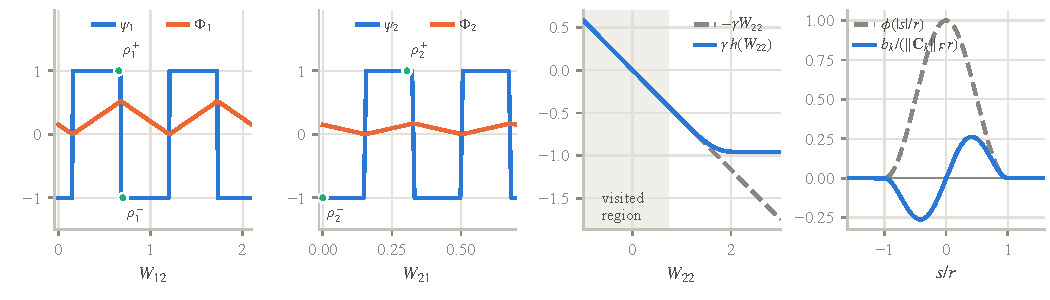
\includegraphics[width=\textwidth]{images/counterexamples/ef21_construction.pdf}
\caption{The components of the objective $\tilde f=g+\sum_k b_k$ of Part~3, as
implemented. \emph{First two panels:} the periodic ramps $\psi_1,\psi_2$ and
their bounded antiderivatives $\Phi_1,\Phi_2$ over two periods; the marked
residues $\rho_i^{+}$ (kept at odd iterates) and $\rho_i^{-}$ (even iterates)
lie on the plateaus where $\psi_i=\pm1$ exactly, so from $t\ge4$ the
off-diagonal gradient entries alternate between $+A$ and $-A$. The drawn
$\psi_i$ is the implementation's ramp; the trajectory samples only the
plateaus, on which any $C^\infty$ choice agrees with it. \emph{Third panel:}
the divergence term $-\gamma W_{22}$ and its bounded replacement
$\gamma\,h(W_{22})$ of Remark~\ref{rem:efsm_bdd}; the two agree on the visited
region $\{W_{22}\le\tfrac7{10}\}$ (shaded), so the floor changes no iterate
while restoring Assumption~\ref{as:1}. \emph{Fourth panel:} the correction
$b_k$ of \eqref{eq:bump} along the ray
$\mathbf Z_k+s\,\mathbf C_k/\|\mathbf C_k\|_F$, normalized by
$\|\mathbf C_k\|_F\,r$, with the cutoff $\phi$: $b_k$ vanishes at $\mathbf Z_k$
while $\nabla b_k(\mathbf Z_k)=\mathbf C_k$, and its support, the ball
$\{\|\mathbf W-\mathbf Z_k\|_F\le r\}$, contains no iterate other than its own
center.}
\label{fig:ef21_construction}
\end{figure*}

\emph{The corrections} pin the first three gradients. Fix once a $C^\infty$
cutoff $\phi\colon\mathbb R\to[0,1]$ with $\phi\equiv1$ on $[0,\tfrac12]$ and
$\phi\equiv0$ on $[1,\infty)$, put $r=\tfrac1{50}$, and set
\begin{equation}\label{eq:bump}
b_k(\mathbf W)=\bigl\langle\mathbf C_k,\,\mathbf W-\mathbf Z_k\bigr\rangle\,
\phi\!\bigl(\|\mathbf W-\mathbf Z_k\|_F/r\bigr),
\end{equation}
centered at the first three iterates (from Lemma~\ref{lem:efsm_cycle})
\[
\mathbf Z_1=\mathbf 0,\quad
\mathbf Z_2=\tfrac1{10}\smat{7}{-7}{7}{7},\quad
\mathbf Z_3=\tfrac1{20}\smat{7}{-7}{7}{7}.
\]
Each $b_k$ is $C^\infty$, supported in $\{\|\mathbf W-\mathbf Z_k\|_F\le r\}$;
since its linear factor vanishes at $\mathbf Z_k$ while $\phi(0)=1$,
$\nabla b_k(\mathbf Z_k)=\mathbf C_k$. We choose
$\mathbf C_k:=\hat{\mathbf G}_k-\nabla g(\mathbf Z_k)$ with the explicit
$\hat{\mathbf G}_k$ of \eqref{eq:transient} below, so that
$\nabla\tilde f(\mathbf Z_k)=\hat{\mathbf G}_k$. Every term of $\tilde f$ has a
bounded Hessian, so $\tilde f$ is $C^\infty$ and $\tilde L$-smooth for a finite
$\tilde L(\mu,\text{variant})$.

\begin{lemma}[Realization]\label{lem:efsm_realize}
For every $\mu\in[0,1)$ and either variant, EF21-SignMuon on this $\tilde f$
($\eta=1$, from $\mathbf 0$) generates exactly the targets
\eqref{eq:target_seq}.
\end{lemma}
\paragraph{Proof.}
\emph{The required gradients.} The buffer recursion
$\mathbf M_t=\mu\mathbf M_{t-1}+(1-\mu)\mathbf G_t$ of \eqref{eq:signa_general}
can be solved for the gradients: prescribing the buffers $(\mathbf M_t)_{t\ge1}$
forces $\mathbf G_t=(\mathbf M_t-\mu\mathbf M_{t-1})/(1-\mu)$, and these are
the gradients the function must deliver. Define accordingly the
\emph{transient gradients}
\begin{equation}\label{eq:transient}
\hat{\mathbf G}_t=\frac{\mathbf M_t-\mu\mathbf M_{t-1}}{1-\mu}\quad(t=1,2,3;\ \mathbf M_0=\mathbf 0)
\end{equation}
and the \emph{field gradient}
$\mathbf G^{\pm}=\smat{0}{\pm A}{\pm A}{-\gamma}$, where the prescribed buffer
values $\mathbf M_{1,2,3}$ are given below. With
$\bar{\mathbf M}^{\pm}=\smat{0}{\pm1}{\pm1}{-\gamma}$, the factorization
\begin{equation}\label{eq:polarM}
\begin{gathered}
\bar{\mathbf M}^{\pm}
=\bar{\mathbf D}^{\pm}\,\smat{24/25}{\mp7/25}{\mp7/25}{337/300}\\
(\text{second factor }\succ0,\ \det=1)
\end{gathered}
\end{equation}
shows $\operatorname{polar}(\bar{\mathbf M}^{\pm})=\bar{\mathbf D}^{\pm}$, with
singular values $\tfrac34$ and $\tfrac43$; this is the condition number
$\tfrac{16}9$ cited in the proof idea.

\emph{Standard momentum} ($\tilde{\mathbf M}_t=\mathbf M_t$). Take
$\mathbf M_1=\mathbf S_1$, $\mathbf M_2=\mathbf S_2$,
$\mathbf M_3=\bar{\mathbf M}^{-}$; then $\hat{\mathbf G}_{1,2,3}$ are the
explicit matrices \eqref{eq:transient}. Feeding $\mathbf G^{(-1)^t}$ for $t\ge4$
keeps $\mathbf M_t=\bar{\mathbf M}^{(-1)^t}$, because
$(1-\mu)\mathbf G^{\pm}=\bar{\mathbf M}^{\pm}-\mu\bar{\mathbf M}^{\mp}$ with $A$
as in \eqref{eq:Amu}. As $\operatorname{polar}(\mathbf S_1)=\mathbf S_1$
(orthogonal) and $\operatorname{polar}(\mathbf S_2)=\mathbf S_2$ (rank one),
\eqref{eq:polarM} yields the targets \eqref{eq:target_seq}.

\emph{Nesterov momentum} ($\tilde{\mathbf M}_t=(1+\mu)\mathbf M_t-\mu\mathbf M_{t-1}$).
It is here that the orthogonality of $\mathbf S_1$ is needed. The Nesterov
direction involves two consecutive buffers, so prescribing the tail $t\ge4$
already fixes $\mathbf M_3$, and only the preamble remains to absorb the
mismatch at $t=3$; and the set of matrices with a given polar factor
$\mathbf D$ is $\{\mathbf D\mathbf H:\mathbf H\succ0\}$, which is
three-dimensional when $\mathbf D$ is orthogonal but only one-dimensional (a
positive scalar) when $\mathbf D$ has rank one. A preamble of two rank-one
targets leaves too little freedom: a symbolic check shows that it admits no
realization once $\mu\gtrsim0.3$. One orthogonal target supplies enough
freedom, of which the construction uses a single scalar, the $\tau$ below.
Take $\mathbf M_1=\tfrac1{1+\mu}\mathbf S_1\mathbf H_1$,
$\mathbf M_2=\tfrac1{1+\mu}(\mathbf S_2+\mu\mathbf M_1)$,
$\mathbf M_3=\bar{\mathbf M}'^{-}$ and $\mathbf M_t=\bar{\mathbf M}'^{(-1)^t}$
($t\ge4$), where $\bar{\mathbf M}'^{\pm}=\smat{0}{\pm\nu}{\pm\nu}{-\gamma}$,
$\mathbf H_1=\operatorname{diag}(1,1+\tau)$, and, for $\mu>0$,
\[
\tau=\Bigl(\tfrac{140(1+\mu)^2}{1+2\mu}-44\Bigr)\tfrac{1+\mu}{117\mu}>0 .
\]
(At $\mu=0$ the Nesterov rule reads $\tilde{\mathbf M}_t=\mathbf M_t$ and is the standard case already treated, so nothing is left to prove there.)
Then $\tilde{\mathbf M}_1=\mathbf S_1\mathbf H_1$ and
$\tilde{\mathbf M}_2=\mathbf S_2$ have polar factors $\mathbf S_1,\mathbf S_2$,
and $\tilde{\mathbf M}_t=\bar{\mathbf M}^{(-1)^t}$ for $t\ge4$ (since
$\nu(1+2\mu)=1$). The one nontrivial step is $t=3$. Set
$\mathbf H_3:=\bar{\mathbf D}^{-}\tilde{\mathbf M}_3$; since
$(\bar{\mathbf D}^{-})^2=\mathbf I$, this is the same as
$\tilde{\mathbf M}_3=\bar{\mathbf D}^{-}\mathbf H_3$. The stated $\tau$ is
exactly the value making $\mathbf H_3$ symmetric,
and $\mathbf H_3\succ0$ for all $\mu\in(0,1)$: under $\mu=\tfrac{s}{1+s}$ ($s>0$)
the numerators of its two leading minors are polynomials in $s$ with
nonnegative coefficients. Hence
$\operatorname{polar}(\tilde{\mathbf M}_3)=\bar{\mathbf D}^{-}$, completing
\eqref{eq:target_seq}.

\emph{The function delivers these gradients.} It remains to verify
$\nabla\tilde f(\tilde{\mathbf X}_{t-1})=\hat{\mathbf G}_t$ for $t\le3$ and
$=\mathbf G^{(-1)^t}$ for $t\ge4$, by induction along the run: as long as the
gradients match this prescription, the iterates are those computed in
Part~2, and the prescription need only be checked at those points. By
Lemma~\ref{lem:efsm_cycle} the iterates
$\tilde{\mathbf X}_0,\tilde{\mathbf X}_1,\tilde{\mathbf X}_2$ are exactly the
centers $\mathbf Z_1,\mathbf Z_2,\mathbf Z_3$, where
$\nabla\tilde f=\hat{\mathbf G}_{1,2,3}$ by construction. The three balls are
disjoint ($\|\mathbf Z_j-\mathbf Z_k\|_F\ge\tfrac7{10}>2r$), and every later
iterate has $(1,2)$-entry $\ge\tfrac{131}{200}$ while the centers have it
$\le0$, so no ball is re-entered. For $t\ge4$ the query lies in the field,
where
\[
\nabla g(\mathbf W)=\begin{pmatrix}0 & A\psi_1(W_{12})\\ A\psi_2(W_{21}) & -\gamma\end{pmatrix}.
\]
The period shift $\tilde{\mathbf X}_{t+2}-\tilde{\mathbf X}_t
=-(\mathbf d_A+\mathbf d_B)$ advances $W_{12}$ by exactly $+p_1$ and $W_{21}$
by exactly $-p_2$ per period, so the two coordinates travel to $+\infty$ and
$-\infty$ respectively while, mod $p_i$, they hold the residues $\rho_i^{+}$
at odd indices and $\rho_i^{-}$ at even ones; there $\psi_i=\pm1$, giving
$\nabla g=\mathbf G^{(-1)^t}$. $\blacksquare$

\paragraph{Proof of Theorem~\ref{th:ef_div}.}
By Lemma~\ref{lem:efsm_realize} the normalized run produces the targets
\eqref{eq:target_seq}, so by Lemma~\ref{lem:efsm_cycle} its estimate locks onto
the wrong-sign cycle and $\tilde{\mathbf X}_{t+2}-\tilde{\mathbf X}_t$ is a
constant shift. Along it $\Phi_1,\Phi_2$ return to their values and the
corrections $b_k$ vanish, so only the linear term acts:
$\tilde f(\tilde{\mathbf X}_{t+2})-\tilde f(\tilde{\mathbf X}_t)
=-\gamma(-\tfrac7{20})=\tfrac{49}{240}>0$. By Lemma~\ref{lem:efsm_reduction},
$f$ then obeys \eqref{eq:exact_rate_app} with $c=\tfrac{49}{240\tilde L}$. As
$(L,\eta,\mu,\text{variant})$ were arbitrary, no rule $\eta=\eta(L,\mu)$ can
prevent divergence. $\blacksquare$

\begin{remark}[Boundedness below]\label{rem:efsm_bdd}
Only the linear term $-\gamma W_{22}$ makes $\tilde f$ unbounded below, and only
as $W_{22}\to+\infty$, a region the iterates never enter, since
$(\tilde{\mathbf X}_t)_{22}\le\tfrac7{10}$ throughout (it decreases after the
transient). Replacing $-\gamma W_{22}$ by any $C^\infty$ function that agrees
with it on $\{W_{22}\le1\}$ and is constant on $\{W_{22}\ge2\}$ therefore leaves
the whole trajectory, and \eqref{eq:exact_rate_app} with it, unchanged while rendering
$\tilde f$ bounded below (Assumption~\ref{as:1}); the theorem is stated with
this modification in force.
\end{remark}

\begin{figure*}[t]
\centering
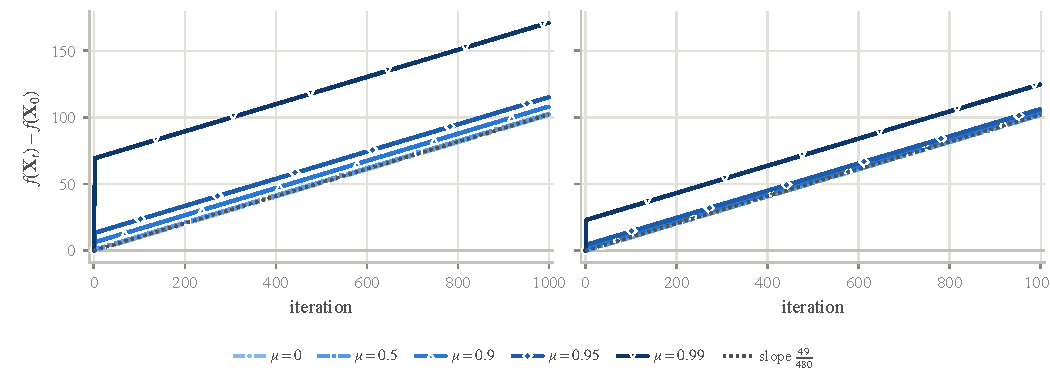
\includegraphics[width=\textwidth]{images/counterexamples/ef21_signmuon_momentum.pdf}
\caption{Momentum does not prevent the divergence of EF21-SignMuon. For each momentum coefficient
$\mu$ and variant, EF21-SignMuon is run on the corresponding instance of
Theorem~\ref{th:ef_div} and $f(\mathbf X_t)-f(\mathbf X_0)$ is plotted;
\emph{left:} standard momentum, \emph{right:} Nesterov. Every setting diverges
at the common rate $\tfrac{49}{480}$ (dotted). Subtracting $f(\mathbf X_0)$
removes the only genuinely $\mu$-dependent offset (the field constant $A(\mu)$
scales a bounded periodic term); what remains is a bounded transient, largest as
$\mu\to1$, on top of the shared linear divergence.}
\label{fig:ef21_momentum}
\end{figure*}

\begin{remark}[The construction is not convex]\label{rem:efsm_nonconvex}
Theorems~\ref{th:1}--\ref{th:3} run on a linear, hence convex, objective;
$\tilde f$ is nonconvex, through the periodic terms $A\Phi_i$ and the
corrections $b_k$. The nonconvexity is forced by the run rather than chosen by
the realization: along the divergent trajectory,
\[
\bigl\langle\nabla\tilde f(\tilde{\mathbf X}_6)-\nabla\tilde f(\tilde{\mathbf X}_3),\
\tilde{\mathbf X}_6-\tilde{\mathbf X}_3\bigr\rangle=-\tfrac{9A}{50}<0,
\]
violating the gradient monotonicity that every convex function obeys, so
\emph{no} convex function generates these iterates and gradients. The theorem
is stated under Assumptions~\ref{as:1}--\ref{as:2} because that is where it is
needed: EF21-MuonUSign and EF21-MuonSign converge under exactly these
hypotheses (Theorem~\ref{thm:conv}), so the divergence and the guarantees
concern one problem class. Whether some convex instance, necessarily through a
different trajectory, also defeats EF21-SignMuon we leave open.
\end{remark}

\begin{remark}[Verification]\label{rem:efsm_scope}
The construction is checked in two independent ways: symbolically, in exact
rational arithmetic, and numerically, by running the float64 reference
implementation of Algorithm~\ref{ef21_signmuon} on the assembled $\tilde f$.
The right panel of Figure~\ref{fig:divergence_plot} confirms that at $\mu=0$
EF21-SignMuon is the only one of the eight methods that diverges, the others
(SignMuon, MuonUSign, MuonSign, EF21-MuonUSign, EF21-MuonSign, SignSGD, Muon)
staying bounded; Figure~\ref{fig:ef21_momentum} confirms that EF21-SignMuon
diverges at the exact rate $\tfrac{49}{480}$ for every
$\mu\in\{0,\tfrac12,0.9,0.95,0.99\}$ under both standard and Nesterov momentum, as the
reduction predicts.
\end{remark}
